
\section{Implementación}
En este capítulo expondremos la implementacion tanto del servidor como de la aplicación móvil.


\subsection{Servidor}
En capítulos anteriores ya comentamos la estructura de paquetes seguida para desarrollar el servidor, en este hablaremos de JpaRepository.\\

JpaRepository es un repositorio que nos ofrece métodos genéricos de gestión de clases persistentes como también métodos mas concreto que nos permiten realizar operaciones complejas abstrayendonos de su implementacion.

Ademas este repositorio se adapta a la clase con la que va a trabajar.
\begin{lstlisting}[language=java,
 ,backgroundcolor=\color{backcolour},   
    commentstyle=\color{codegreen},
    keywordstyle=\color{magenta},
    numberstyle=\tiny\color{codegray},
    stringstyle=\color{codepurple}]
    
public interface UsuarioRepository 
extends JpaRepository<Usuario, Long> {
		}

\end{lstlisting} 
	




	
Como se puede ver en la figura anterior, este interfaz importa la clase Usuario accediendo a todos sus atributos y generando una lista de métodos para estos atributos concretos como podemos ver en la siguiente.\\

\begin{lstlisting}[language=java,
 ,backgroundcolor=\color{backcolour},   
    commentstyle=\color{codegreen},
    keywordstyle=\color{magenta},
    numberstyle=\tiny\color{codegray},
    stringstyle=\color{codepurple}]
    
public interface UsuarioRepository 
extends JpaRepository<Usuario, Long> {

	public Usuario findByCorreo(String correo);

	public Usuario findByNombre(String nombre);

	public List<Usuario> findByNombreContaining
		(String nombre);

	@Override
	public <S extends Usuario> S save(S usuario);

	@Override
	public void delete(Long idUsuario);

	@Override
	public boolean exists(Long idUsuario);

	@Override
	public <S extends Usuario> S saveAndFlush(S usuario);

	@Override
	public Usuario findOne(Long idUsuario);
	}


\end{lstlisting} 

\newpage

 
 
 
 
 \subsection{Aplicación móvil Android}
En este capítulo comentaremos aspectos concreto de la implementación de de la aplicación móvil.



\subsubsection{Mapas}

 Para la creación de rutas tanto individuales como compartidas como para crear PDI el usuario necesita conocer las coordenadas de los puntos por lo que trascurre su ruta. Para ello necesitamos los mapas de Google Maps y métodos de sus APIs.
 
 
 \begin{lstlisting}[language=java,
 ,backgroundcolor=\color{backcolour},   
    commentstyle=\color{codegreen},
    keywordstyle=\color{magenta},
    numberstyle=\tiny\color{codegray},
    stringstyle=\color{codepurple}]
compile 'com.google.android.gms:play-services-maps:10.2.0'

\end{lstlisting}
 
 Con la dependencia de la figura anterior permitimos a nuestra aplicación que use los servicios de  Google Maps.\\
 Para marcar un punto en el mapa y que este quede visible en el mapa necesitamos implementar un método que capture los clic en el mapa y que nos devuelva las coordenadas del punto marcado.
 
 
 \begin{lstlisting}[language=java,
 ,backgroundcolor=\color{backcolour},   
    commentstyle=\color{codegreen},
    keywordstyle=\color{magenta},
    numberstyle=\tiny\color{codegray},
    stringstyle=\color{codepurple}]
    
mMap.setMyLocationEnabled(true);
mMap.getUiSettings().setCompassEnabled(true);
mMap.setOnMapClickListener(new GoogleMap
	.OnMapClickListener() {
	public void onMapClick(LatLng point) {
	mMap.clear();
	poilongitud = point.longitude;
	poilatitud = point.latitude;
	LatLng Yo = new LatLng(poilatitud, poilongitud);
	Marker mensaje = 
	mMap.addMarker(new MarkerOptions()
		.position(Yo)
		.title("Guardar este punto?"));
  	mensaje.showInfoWindow();
	VerTodosPois();

\end{lstlisting} 
 
 
 
 
  Con el fragmento de código de la figura anterior  se capturaría ese clic y aparecería el Marker común de todos los mapas de Google Maps acompañado del mensaje \textit{"Guardar este punto?"}. En nuestro proyecto personalizamos los Marker de modo que cuando guardamos ese punto pase a a representarse con icono de un pescador o de un cazador dependiendo del PDI que estuviéramos guardando. Para ello usamos el siguiente fragmento de código.

 

\begin{lstlisting}[language=java,
 ,backgroundcolor=\color{backcolour},   
    commentstyle=\color{codegreen},
    keywordstyle=\color{magenta},
    numberstyle=\tiny\color{codegray},
    stringstyle=\color{codepurple}]
    
protected Marker createMarkerPesca(double
		latitude,Double longitude, String nombre,
		String	descripcion) {
       		return mMap.addMarker(new MarkerOptions()
                	.position(new LatLng(latitude, 							longitude))
                	.anchor(0.5f, 0.5f)
                	.title(nombre).snippet(descripcion)
	                .icon(BitmapDescriptorFactory
    	       		.fromResource(R.drawable.pescador)));
    }


\end{lstlisting} 
 
 
 
 Y así es como quedaría en la Figura~\ref{fig:marker}  

 
 
 
	\begin{figure}
\begin{minipage}[b]{0.5\linewidth} %Una minipágina que cubre la mitad de la página
\centering
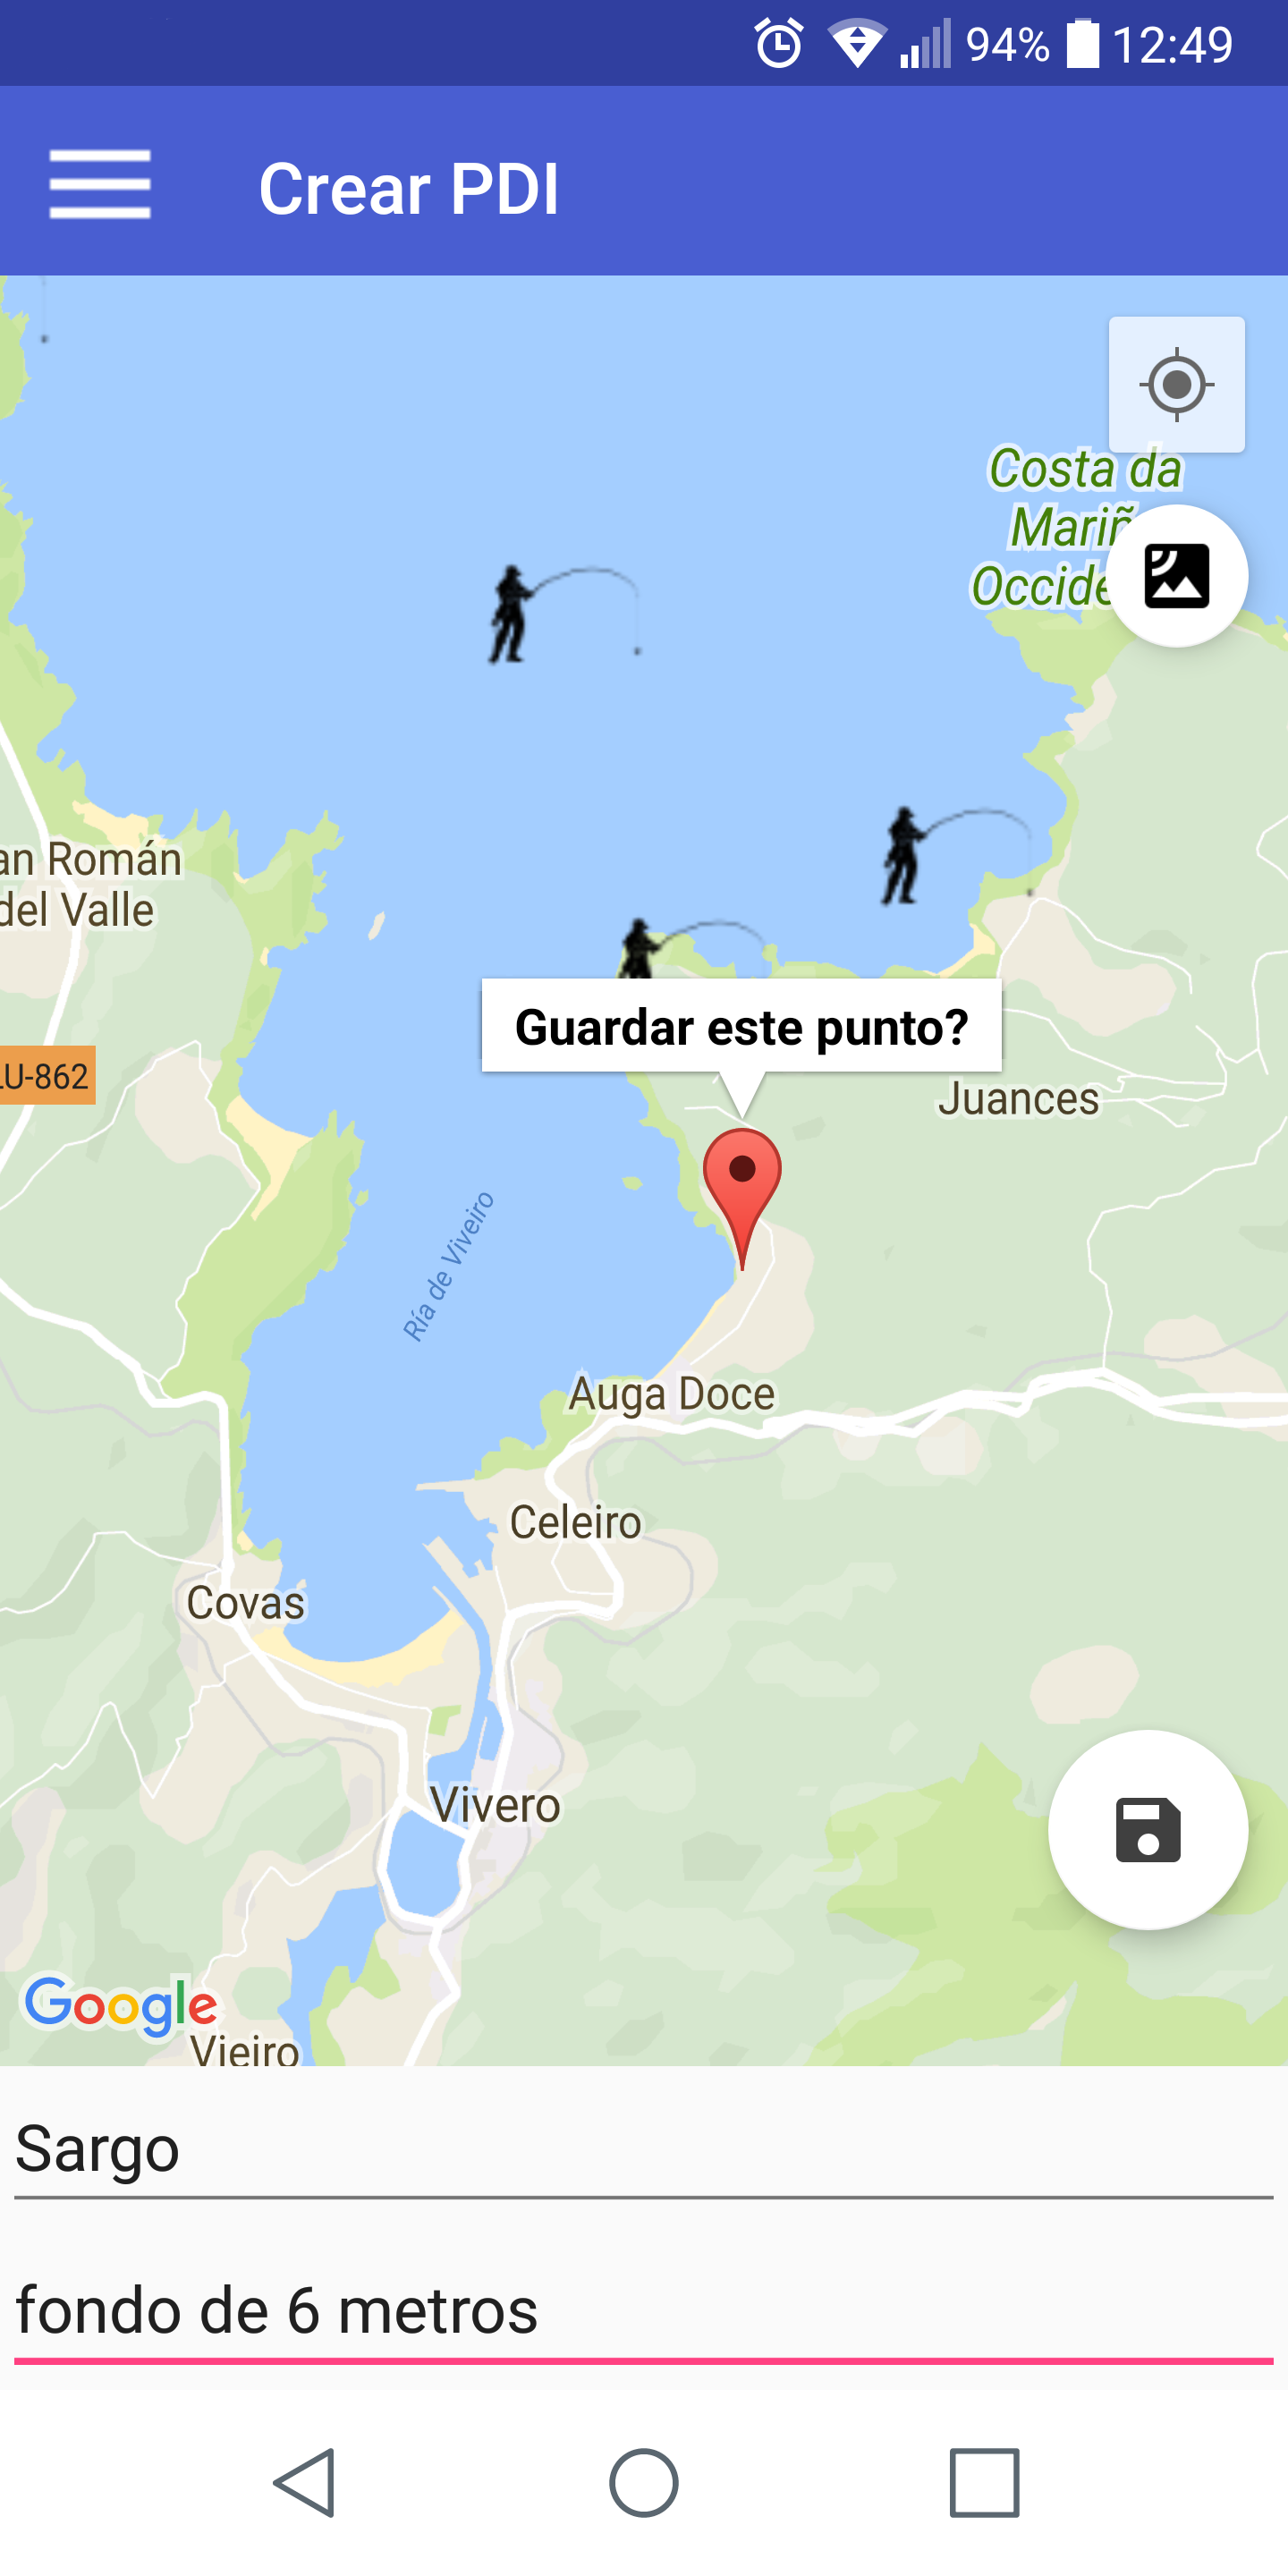
\includegraphics[width=6cm]{capturamovil/pdiguardar.png}
 \label{figura1}
\caption{Marker antes de guardar el PDI}

\end{minipage}
\hspace{0.5cm} % Si queremos tener un poco de espacio entre las dos figuras
\begin{minipage}[b]{0.5\linewidth}
\centering
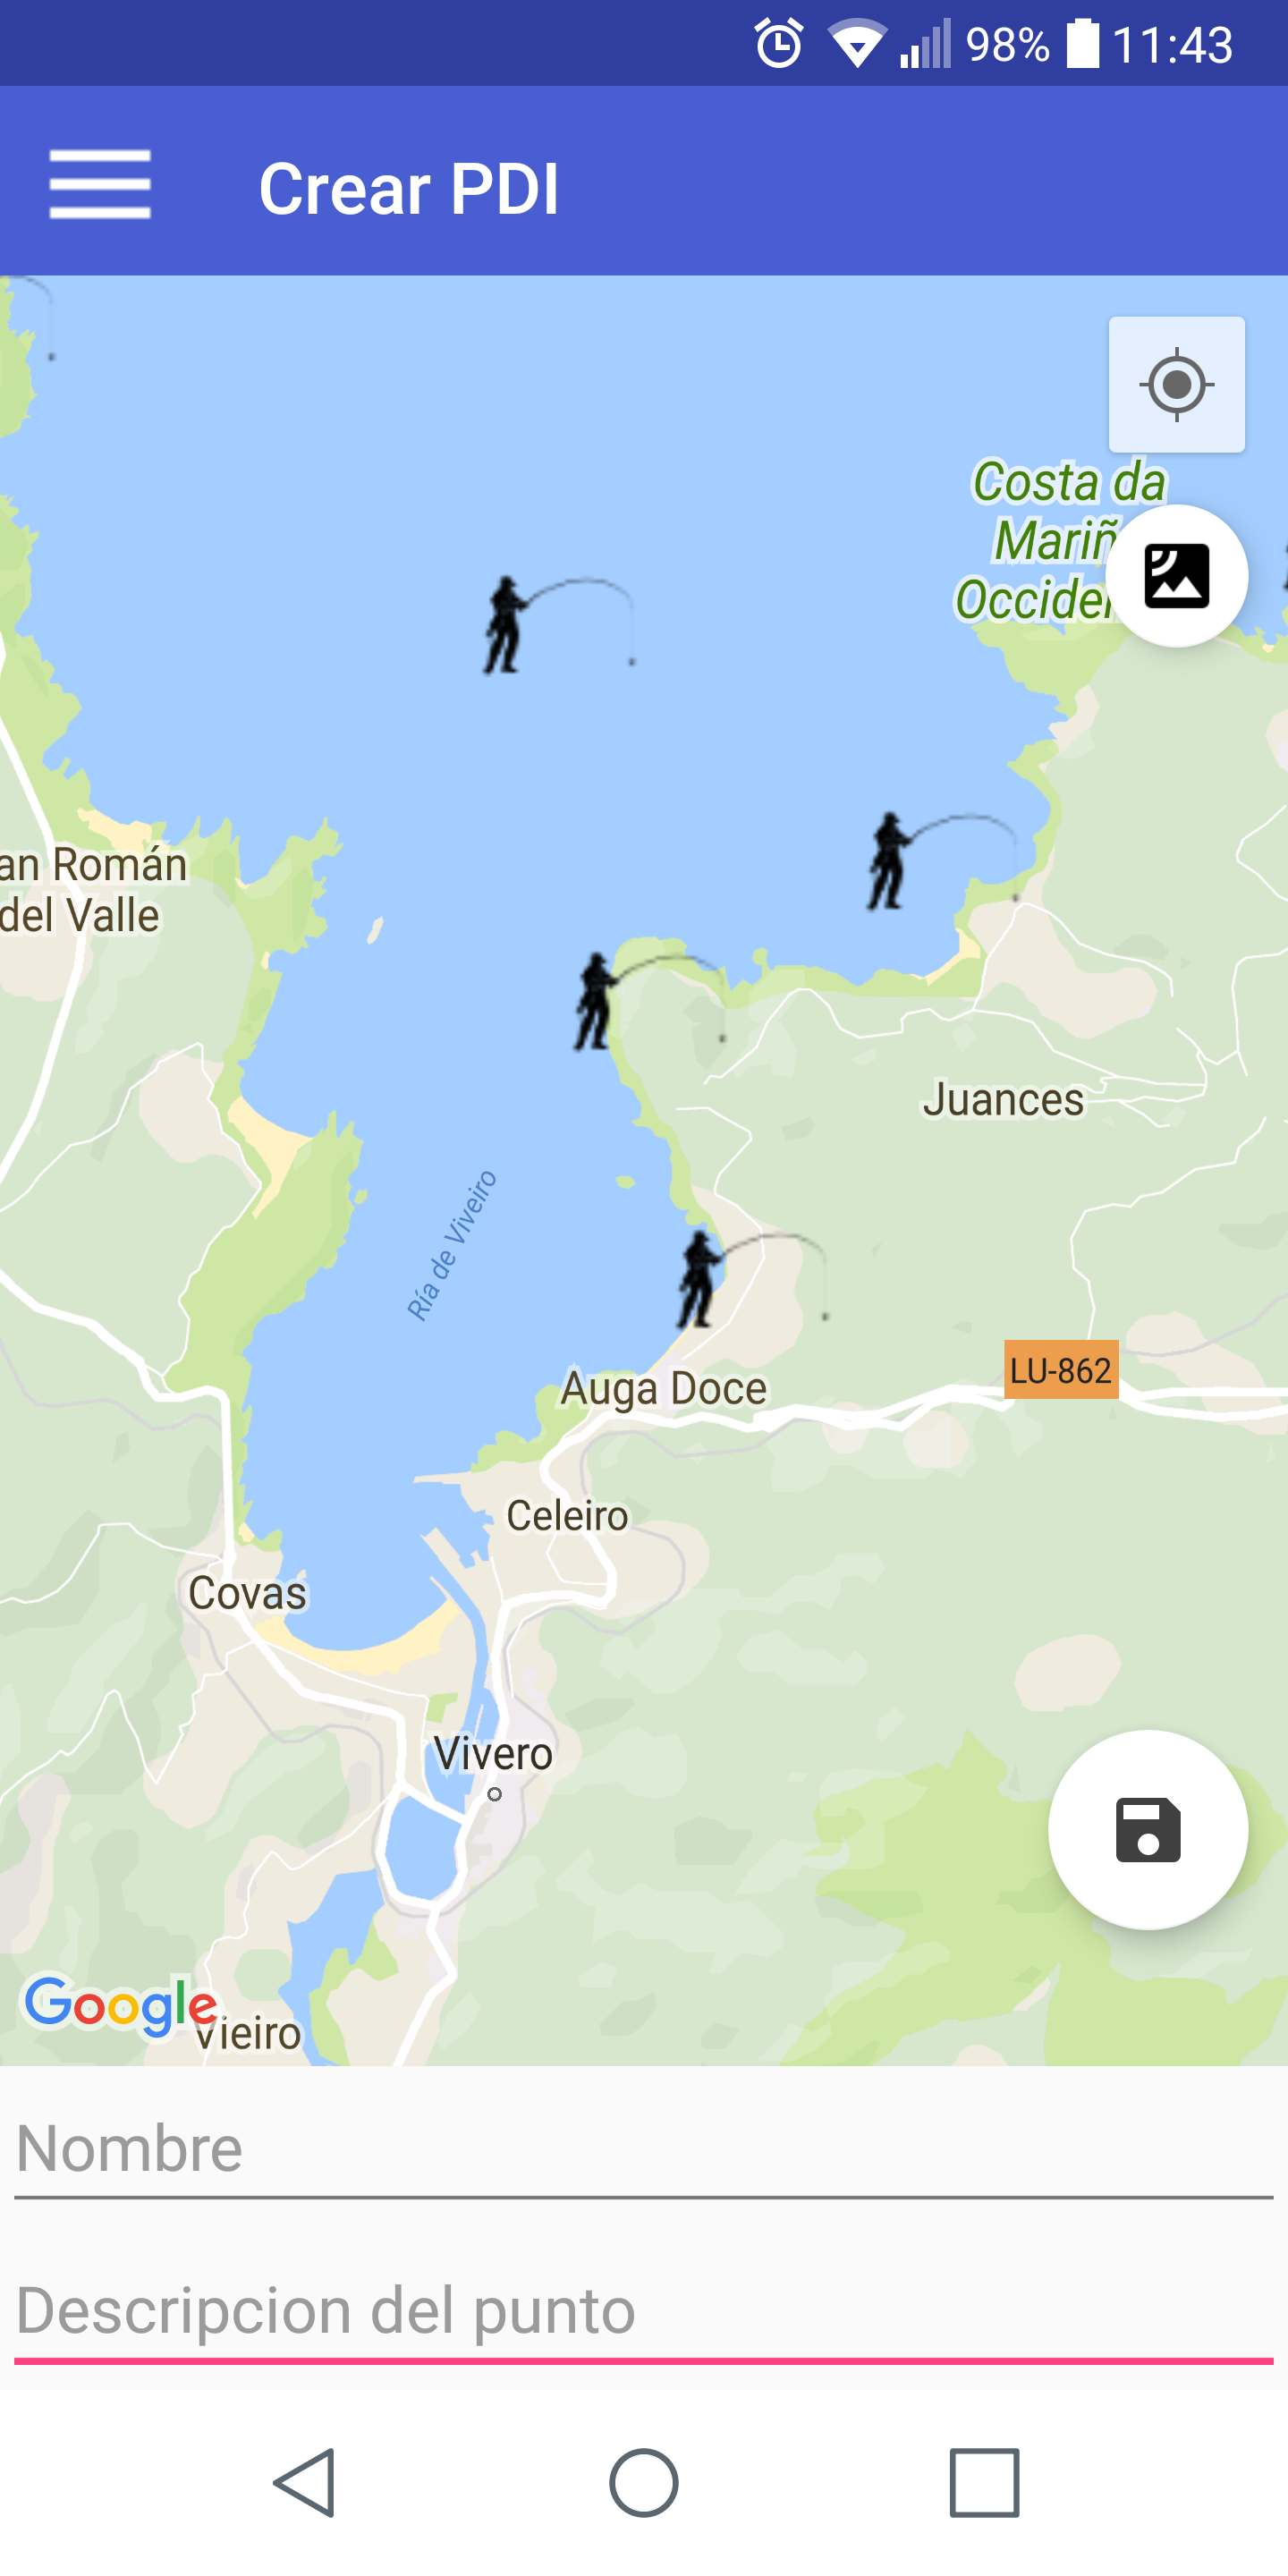
\includegraphics[width=6cm]{capturamovil/pdiguardar2.png}
 \label{figura2}
\caption{Marker después }

\end{minipage}
		\label{fig:marker}

\end{figure} 
 
 
 
 \subsubsection{Localización}
  Para la creación de ruta necesitamos una método que nos proporcione las coordenadas(latitud y longitud) de los puntos por los que trascurre el usuario en la ruta. Para ellos necesitamos la siguiente dependencia.

	
\begin{lstlisting}[language=java,
 ,backgroundcolor=\color{backcolour},   
    commentstyle=\color{codegreen},
    keywordstyle=\color{magenta},
    numberstyle=\tiny\color{codegray},
    stringstyle=\color{codepurple}]
compile 'com.google.android.gms:play-services-location:10.2.0'


\end{lstlisting}	
	
	
	Una vez añadida esta dependencia necesitamos un método que nos proporciones las coordenadas concretas, para ellos usaremos el siguiente fragmento de código.
	
\begin{lstlisting}[language=java,
 ,backgroundcolor=\color{backcolour},   
    commentstyle=\color{codegreen},
    keywordstyle=\color{magenta},
    numberstyle=\tiny\color{codegray},
    stringstyle=\color{codepurple}]
mlocManager.requestLocationUpdates(LocationManager
.GPS_PROVIDER15, 0,(LocationListener) Local);


\end{lstlisting}	

El método ofrece el par de coordenadas cuando el usuario se mueve X metros o bien por un intervalo de tiempo en segundos.


Como se puede observar en la figura anterior en nuestro proyecto indicamos que los segundos que deberían transcurrir para devolver una coordenadas sería de 15.\\
Cuando nosotros estamos realizando la ruta en ocasiones el GPS pierde precisión y sitúa al usuario en punto un tanto lejano, lo cual es imposible ya que no se puede mover tan rápido. Este error del GPS lo hemos resuelto de la siguiente manera.\\



\newpage
\begin{lstlisting}[language=java,
 ,backgroundcolor=\color{backcolour},   
    commentstyle=\color{codegreen},
    keywordstyle=\color{magenta},
    numberstyle=\tiny\color{codegray},
    stringstyle=\color{codepurple}]
      iniTramo = finTramo;
      finTramo = new LatLng(latitud, longitud);
      Location location1 = new Location("localizacion 1");
      location1.setLatitude(iniTramo.latitude);  //latitud
      location1.setLongitude(iniTramo.longitude); //longitud
      Location location2 = new Location("localizacion 2");
      location2.setLatitude(finTramo.latitude);  //latitud
      location2.setLongitude(finTramo.longitude); //longitud
      double distance = location1.distanceTo(location2);
\end{lstlisting}

En este código lo que hacemos es calcular la distancia entre dos puntos consecutivos. Usamos un método que pertenece a la API,  el cual necesita un par de coordenadas. El dato que devuelve viene dado en metros y viene dado tiene en cuenta la curvatura de la tierra para calcularlo. Si esta distancia es superior a 15 metros desechamos ese punto.

\begin{figure}[H]
		\centering
		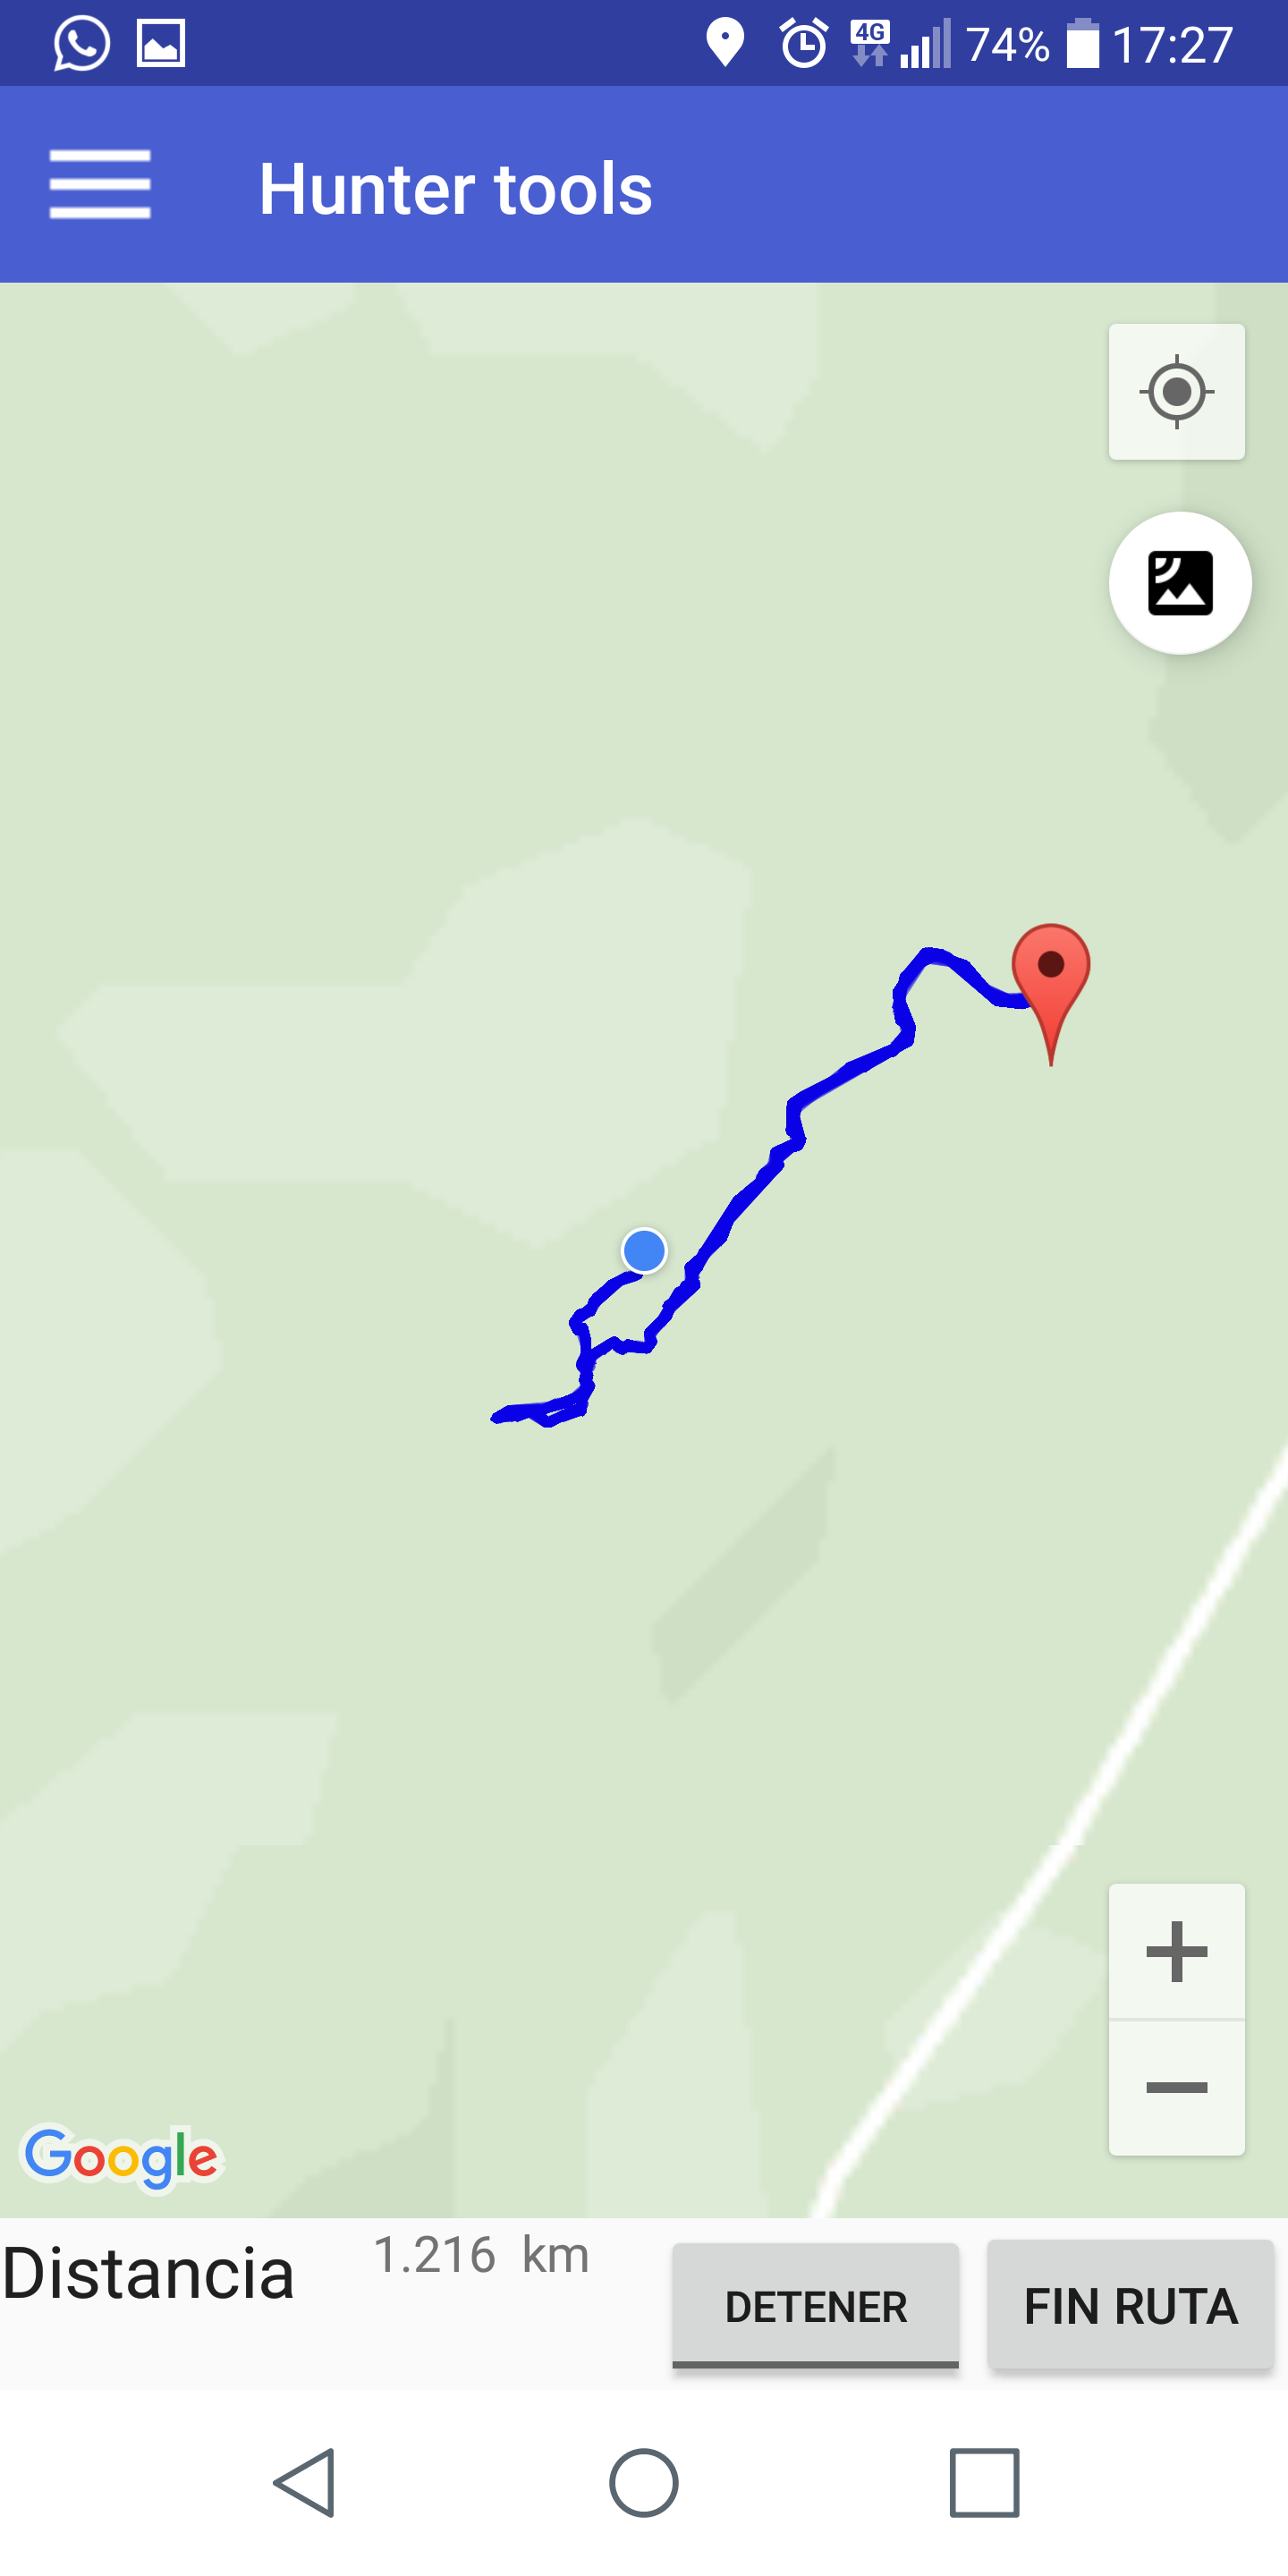
\includegraphics[width=0.4\textwidth] {capturamovil/individual-navegacion.png}
		\caption{Visualización de la ruta mientras se realiza}
	\end{figure}
	
\subsubsection{Firebase} 
Cuando el usuario inicia una ruta compartida el sistema avisa al resto de integrantes de grupo de que acaban de ser invitados a ella, esta acción la realizamos mediante las Notificaciones Push con Firebase. Para ello tenemos que empezar añadiendo las dependencias siguientes.

	\begin{lstlisting}[language=java,
 ,backgroundcolor=\color{backcolour},   
    commentstyle=\color{codegreen},
    keywordstyle=\color{magenta},
    numberstyle=\tiny\color{codegray},
    stringstyle=\color{codepurple}]
 compile 'com.google.firebase:firebase-core:10.2.0'
 compile 'com.google.firebase:firebase-messaging:10.2.0'

\end{lstlisting}
	
Del lado del servidor enviamos una notificación con una serie de campos necesarios para identificar la ruta a un usuario concreto. Este usuario lo identificamos por un token que almacenamos en la base de dato, este token es característico de cada móvil. Para que nuestra aplicación  pueda recibir y entender esta notificación necesitaremos el siguiente fragmento de código.
	\begin{lstlisting}[language=java,
 ,backgroundcolor=\color{backcolour},   
    commentstyle=\color{codegreen},
    keywordstyle=\color{magenta},
    numberstyle=\tiny\color{codegray},
    stringstyle=\color{codepurple}]
 @Override
 public void onMessageReceived(RemoteMessage remoteMessage) {
        Map<String, String> data = remoteMessage.getData();
        titulo= data.get("titulo");
        nombreGrupo= data.get("nombreGrupo");
        accion= data.get("accion");
        idRuta= data.get("idRuta");
        verAccionString ();
        EventBus.getDefault().post(remoteMessage
        .getData().toString());
       
           }

\end{lstlisting}
Este método pasearía el JSON que envía el servidor y guardaría los datos necesario en el móvil.
En la siguiente captura veríamos la notificación en el móvil.	
	
	\begin{figure}[htbp]
\begin{minipage}[b]{0.5\linewidth} %Una minipágina que cubre la mitad de la página
\centering
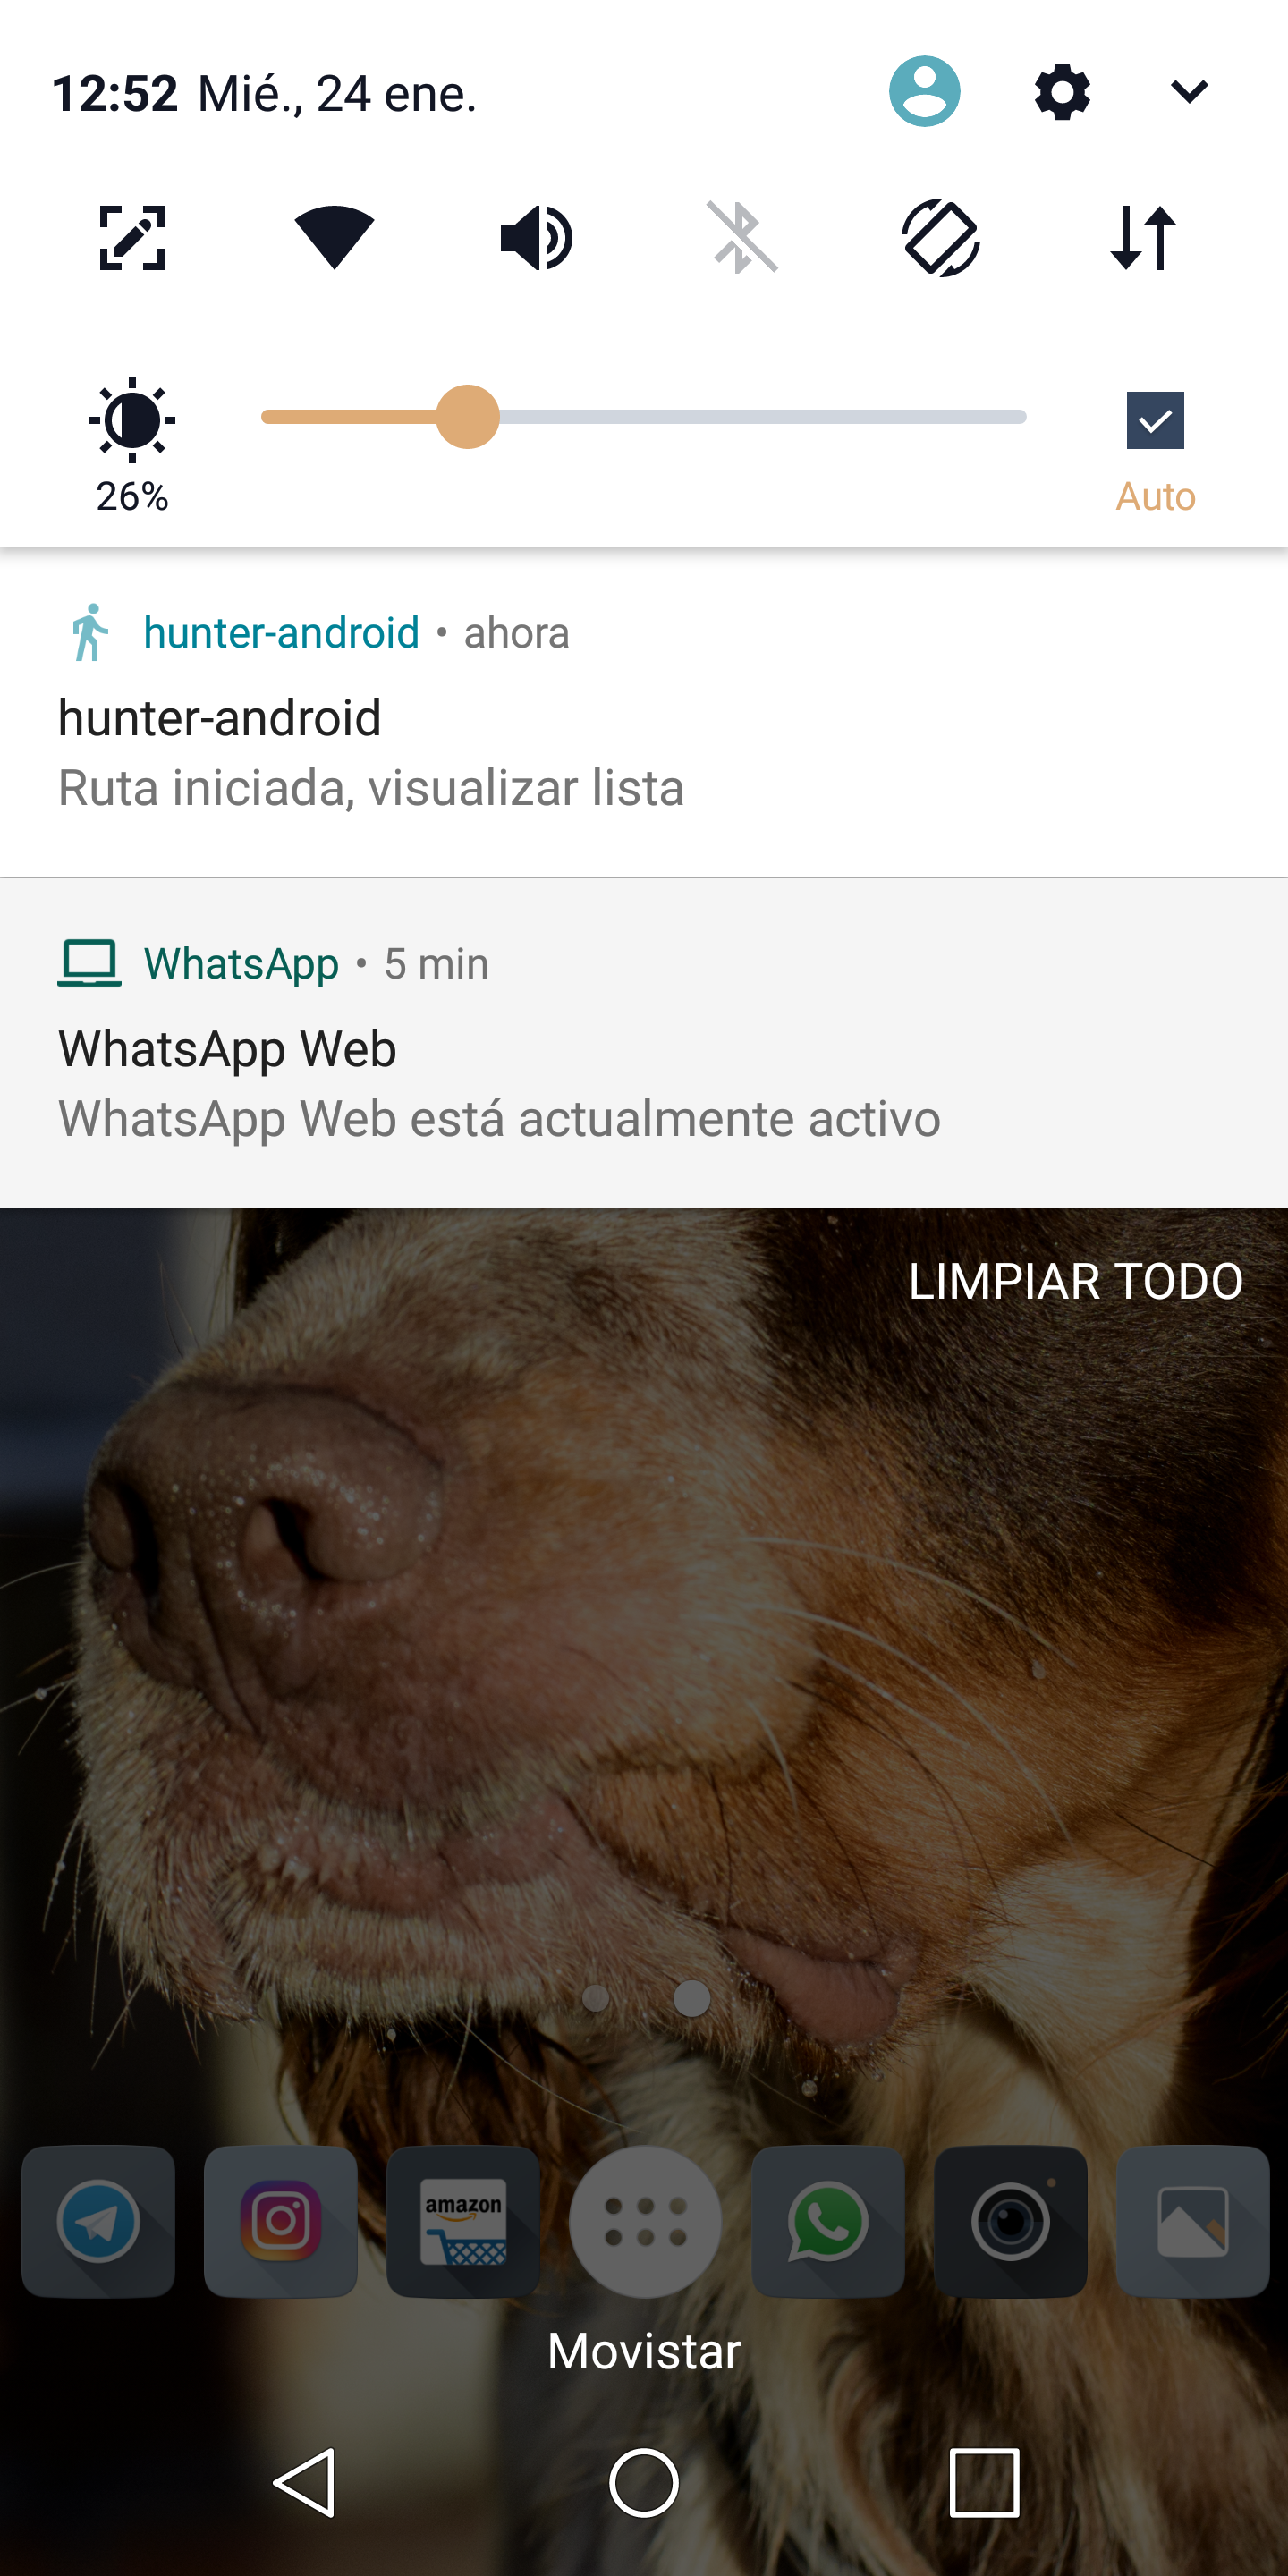
\includegraphics[width=6cm]{capturamovil/push1.png}
 \label{figura1}

\end{minipage}
\hspace{0.5cm} % Si queremos tener un poco de espacio entre las dos figuras
\begin{minipage}[b]{0.5\linewidth}
\centering
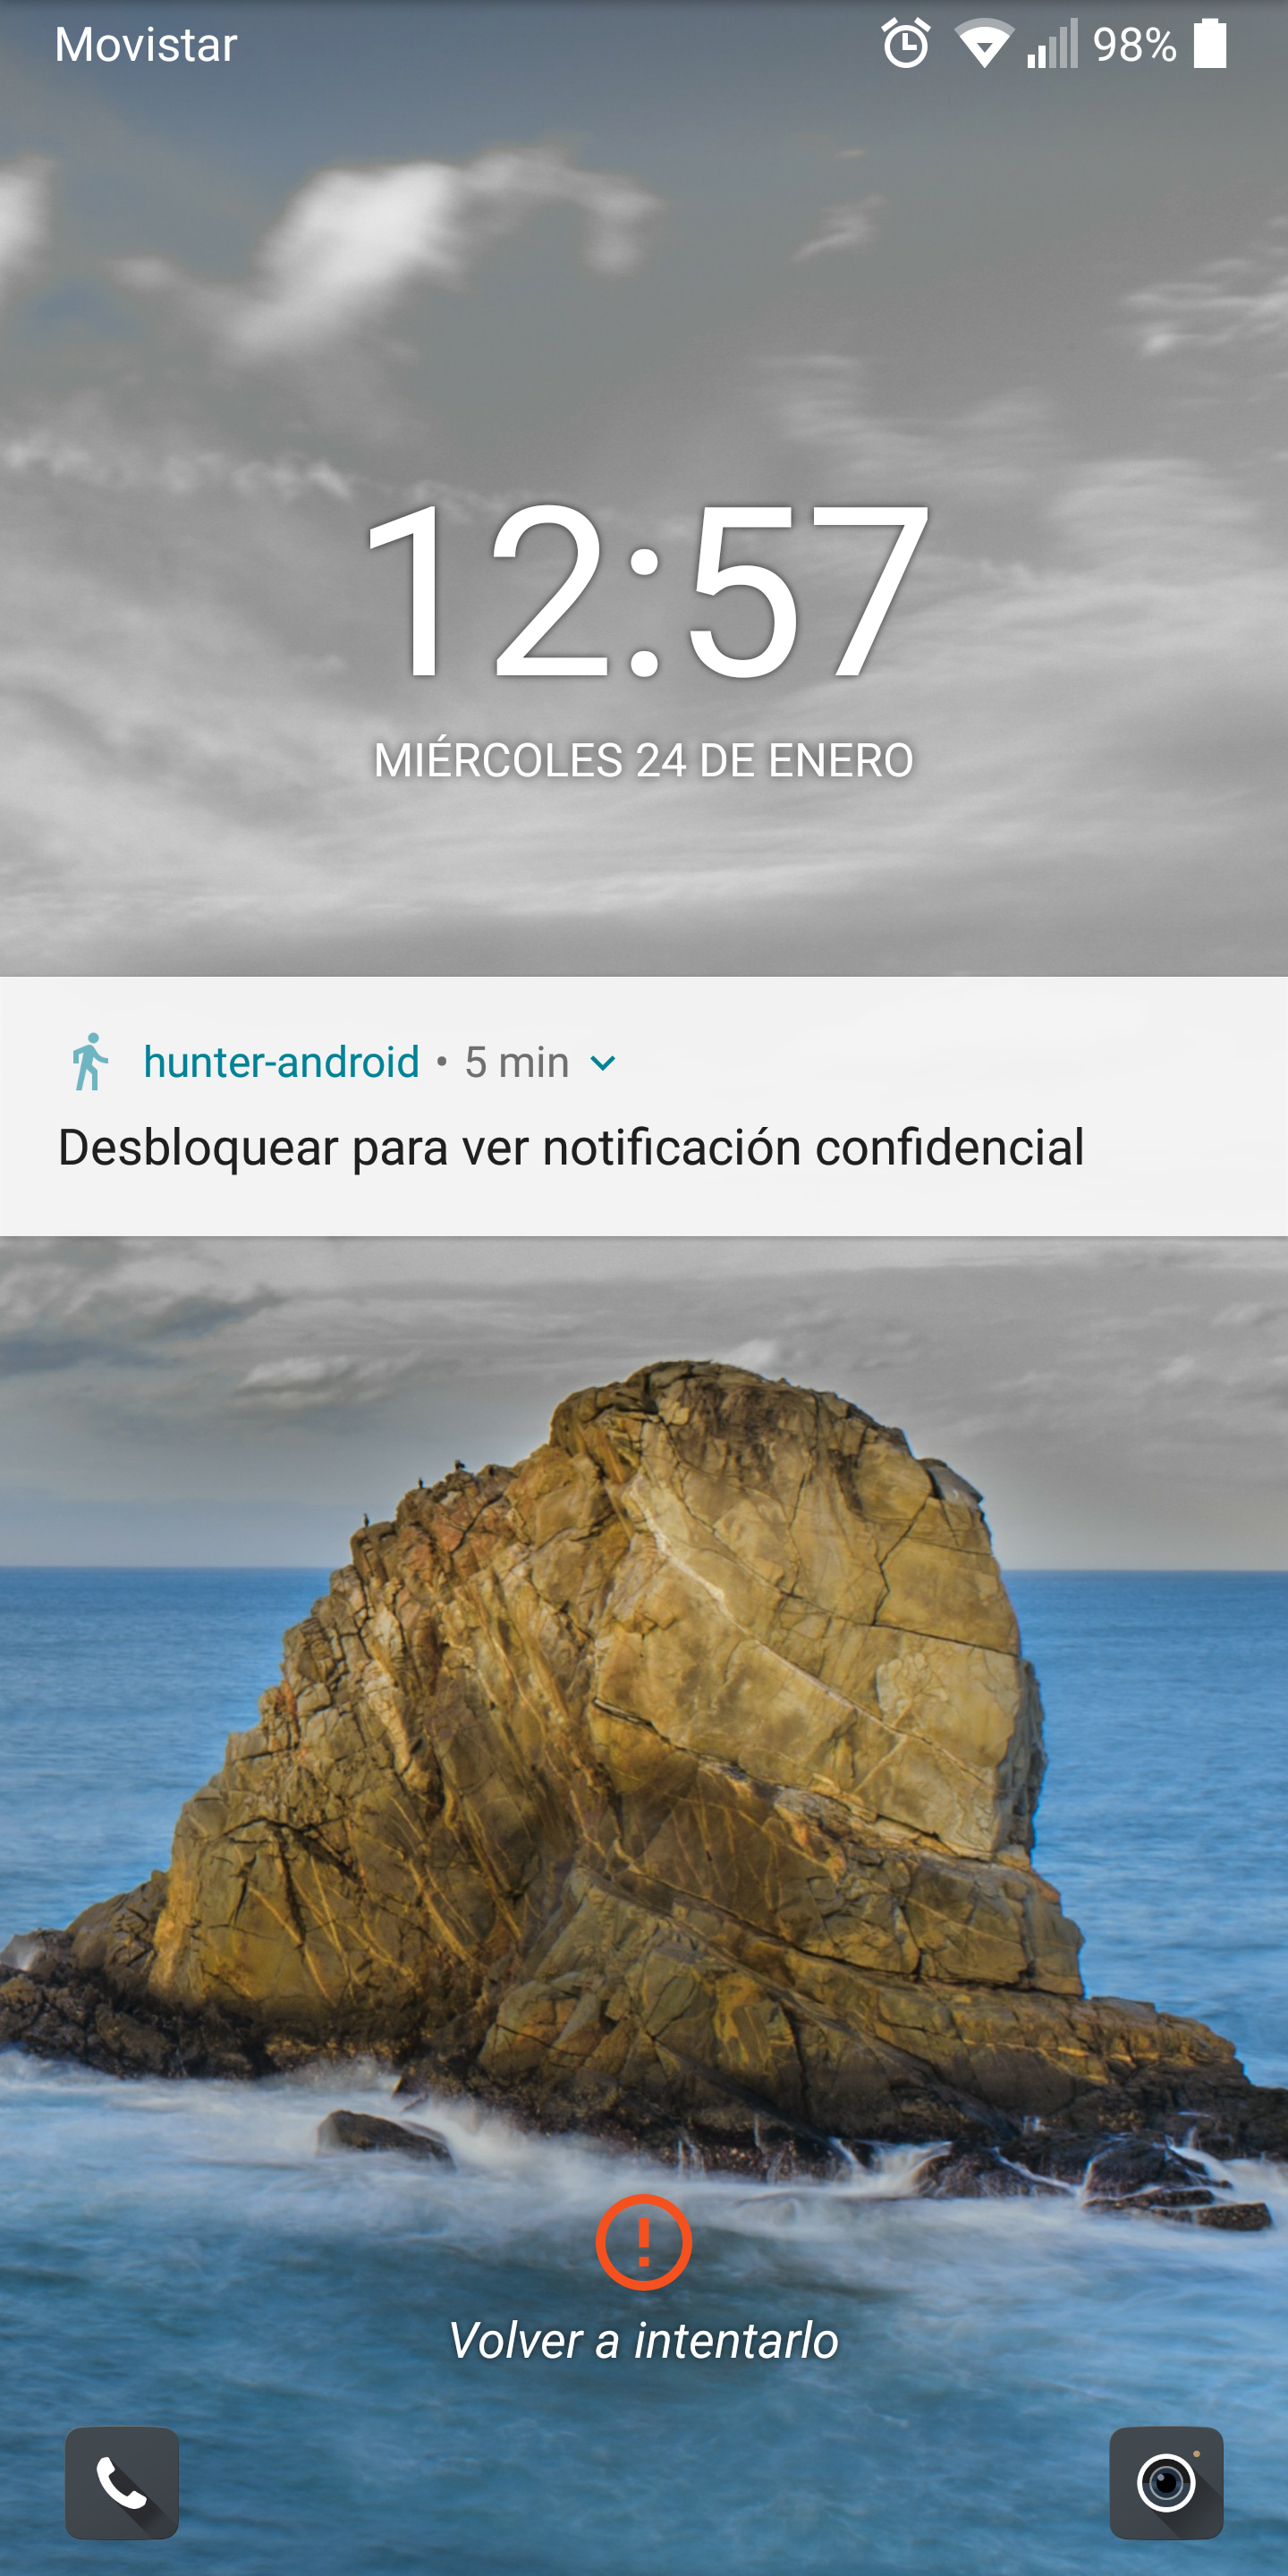
\includegraphics[width=6cm]{capturamovil/push2.png}
 \label{figura2}

\end{minipage}
\caption{Notificación push }
\end{figure} 
 
	
\newpage
	
\section{Pruebas}
Las pruebas son un tema muy importante a tener en cuenta en cualquier proyecto de software. Nos permiten conoces ciertos aspectos que fallan en el sistema de manera objetiva y conocer ciertos riesgos que se nos pasaron por alto en la implementacion.
Dado que usamos la metodología Scrum y como describimos en el capitulo de seguimiento al final de cada Sprint se harán las pruebas para esas historias de usuario.



\subsection{Pruebas de unidad}
Las pruebas de unidad se  encargan de comprobar el  buen funcionamiento de partes de código. Esta comprobación se realiza normalmente a nivel de clase  asegurándonos que el funcionamiento es el adecuado.\\En nuestro caso las pruebas de unidad se realizaron en el servidor ayudándonos del framework de pruebas JUnit. Como ya se comentó JUniT es una tecnología que ayuda a la ejecución de pruebas integrado en nuestro Eclipse Java EE IDE para la comprobación del funcionamiento de métodos o clases.

Como también se usó el framework Spring para el desarrollo este también fue empleado para los test ya que ayuda a la inyección de dependencias y otras gestiones de las transacciones.



\begin{lstlisting}[language=java,
 ,backgroundcolor=\color{backcolour},   
    commentstyle=\color{codegreen},
    keywordstyle=\color{magenta},
    numberstyle=\tiny\color{codegray},
    stringstyle=\color{codepurple}]
@RunWith(SpringJUnit4ClassRunner.class)
@WebAppConfiguration
@Profile("test")
@ContextConfiguration("classpath:root-context.xml")
public class UsuarioServiceTest {

	@Autowired
	private UsuarioService usuarioService;
	
	@Test
	public void testprueba() {

\end{lstlisting}







\subsection{Pruebas de integración y aceptación}
Las pruebas de integración entre los componentes del sistema y las de aceptación se realizaron de forma manual. En ellas se comprobaba el funcionamiento y la respuesta antes las acciones realizadas.\\
Como el servidor estaba desplegado en un servidor de aplicaciones las pruebas se podían realizar de 2 maneras:
\begin{itemize}
\item Mediante el emulador propio de Android.\\
Esta opción fue la utilizada para depurar la aplicación en los primeros Sprint ya que era más cómodo a la hora realizar las pruebas usar el teclado.
\item  Mediante un móvil en el cual se instalaba nuestra aplicación. En cambio esta opción  fue la más utilizada en los últimos Sprints ya que requerían unas pruebas más reales en  lugares abiertos, ya que se perseguía la comprobación de la precisión del GPS  en casos reales de uso. Esto fue clave para mejora de la creación de rutas.
\end{itemize}







